\documentclass{article}
% Add this line for TeX Live
\usepackage{iftex}

% Encodings, page setup, paragraph formatting, font
\usepackage[top=0.9in, bottom=1in, left=1.5in, right=1.5in]{geometry}
\usepackage[icelandic]{babel}
\usepackage[T1]{fontenc}
\usepackage[sc]{mathpazo}
\usepackage[parfill]{parskip}
\usepackage{cancel}
\usepackage{comment}
% Tables and lists
\usepackage{booktabs,tabularx}
\usepackage{multirow}
\usepackage{enumerate}
\usepackage{adjustbox}
\usepackage{multicol}
\usepackage{enumitem}
\usepackage{xcolor}
% Math
\usepackage{amsmath, amsfonts, amssymb, amsthm}
% Graphics
\usepackage{graphicx}
\usepackage{forest}
\usepackage{tikz}
\usetikzlibrary{positioning, shapes, arrows.meta}
% Code environment
\usepackage{listingsutf8}
\definecolor{commentcolor}{RGB}{0, 128, 0} % Grænn
\definecolor{keywordcolor}{RGB}{0, 0, 255}   % Blár
\definecolor{stringcolor}{RGB}{163, 21, 21}      % Dökkrauður
\definecolor{numbercolor}{RGB}{128, 0, 128}      % Fjólublár
\definecolor{identifiercolor}{RGB}{0, 0, 0}      % Svartur

\lstset{
    language=C,
    basicstyle=\ttfamily,
    keywordstyle=\color{keywordcolor}\bfseries,
    commentstyle=\color{commentcolor},
    identifierstyle=\color{identifiercolor},
    stringstyle=\color{stringcolor},   
    showstringspaces=false,
    numbers=left,
    numberstyle=\tiny\color{gray},
    tabsize=2,
    breaklines=true,
    columns=fullflexible,
    keepspaces=true,
    inputencoding=utf8, 
    extendedchars=true,  
    literate=
        {á}{{\'a}}1
        {ð}{{\dh}}1
        {é}{{\'e}}1
        {í}{{\'i}}1
        {ó}{{\'o}}1
        {ú}{{\'u}}1
        {ý}{{\'y}}1
        {þ}{{\th}}1
        {æ}{{\ae}}1
        {ö}{{\"o}}1
        {Á}{{\'A}}1
        {Ð}{{\DH}}1
        {É}{{\'E}}1
        {Í}{{\'I}}1
        {Ó}{{\'O}}1
        {Ú}{{\'U}}1
        {Ý}{{\'Y}}1
        {Þ}{{\TH}}1
        {Æ}{{\AE}}1
        {Ö}{{\"O}}1,
}

% Restin af forskriftinni
\usepackage[pdftex,bookmarks=true,colorlinks=true,pdfauthor={Hafsteinn Einarsson},linkcolor=blue,urlcolor=blue]{hyperref}

% Hyphenation
\hyphenpenalty=5000
% Page and section numbering
\setcounter{secnumdepth}{-1} 
\pagenumbering{gobble}

\title{Tölvutækni og forritun Lokapróf}
\author{brj46 }
\date{Nóvember 2024}

\begin{document}

\maketitle

\vspace{5em}

\begin{center}
    
\includegraphics[scale = 0.2]{myndir/study.png}
\end{center}

\newpage

\section{Hvað þarf ég að kunna fyrir prófið?}

\begin{itemize}
    \item[$\square$] Bitavinnsla með heiltölur (signed og unsigned)
    \item[$\square$] Einfaldar fleytitölur
    \item[$\square$] Skrifa C kóða út frá smalamálskóða (reikniaðgerðir, styriskipanir, föll, bestun,...)
    \item[$\square$] Minnisyfirflæði (buffer overflow)
    \item[$\square$] Skyndiminni (Skipulag og notkun)
    \item[$\square$] Frabrigði, ferlar (fork, wait)
    \item[$\square$] Skipulag á sýndarminni
    \item[$\square$] Minnisúthlutun
\end{itemize}

\section {Hlutir til að setja á minnið}
\begin{itemize}
    \item \textbf{mov}: mov (move) flytur gildi á milli minnisstaða, t.d. \textbf{movl \%eax, \%ebx} flytur gildið í \textbf{\%eax} yfir í \textbf{\%ebx}
    \item \textbf{lea}: lea (load effective address) er notað til að reikna út minnisstaða og setja hana í register, t.d. \textbf{leaq (\%rbx, \%rcx, 4), \%rax} 
    reiknar út \textbf{rbx + (rcx * 4)} og setur í \textbf{\%rax}
    \item q: q stendur fyrir quadword sem er 64 bita gildi
    \item l: l stendur fyrir long sem er 32 bita gildi
    \item w: w stendur fyrir word sem er 16 bita gildi
    \item b: b stendur fyrir byte sem er 8 bita gildi
    \item \%rax: 64 bita register
    \item \%eax: 32 bita register
    \item \%ax: 16 bita register
    \item \%al: 8 bita register
    \item \textbf{Diane's Silk Dress Costs 89} (rdi, rsi, rdx, rcx, r8, r9)
\end{itemize}






\newpage

\section{Tekið frá Tuma}

\subsection{assembly}



\subsection{Uppbrot Gistis}

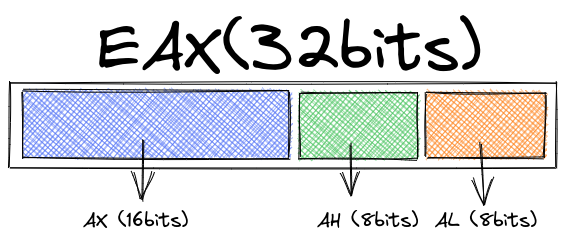
\includegraphics[scale = 0.8]{myndir/gistabrot.excalidraw.png}

\subsection{algengar skipanir}

\begin{tabularx}{\textwidth}{|l|l|X|}
\hline
    \textbf{skipun} & \textbf{argument} & \textbf{lýsing} \\ \hline
    mov & x, y & færir úr x yfir í y, sjá conditional move fyrir neðan\\ \hline 
    push & x & ýtir x á hlaða og eftir að hækka \text{\%ESP} um sizeof(x) bæti og sett þar inn \\ \hline
    pop & x & skilar síðasta gildi sem var sett á hlaðann inn í x \\ \hline
    lea & (x), y & lea, betur þekkt sem leaq er notað til að framkvæma reikning (x) og setja útkomu inn í y \\ \hline
    (x,y) & &skilar útkomu úr reikningi x + y \\ \hline
    0,(,x,y) & & skilar útkomu úr reikningi x * y \\ \hline
    (x,y,z) & & skilar útkomu úr reikningi x + y * z \\ \hline
    2(x, y, z) & & skilar útkomu úr reikningi (2 + (x + y * z)) \\ \hline
    sar & x, y & hliðrar y um x bita til hægri, basically heiltöludeiling með x\\ \hline
    sal & x, y & næstum eins og sar nema til vinstri, núna með margföldun með $2^x$ \\ \hline
    sub & x,y & dregur y frá x \\ \hline
    inc/dec & x & hækkar/lækkar gildi x um 1\\ \hline
\end{tabularx}

ath. \textbf{SHL} og \textbf{SAL} gera það sama en \textbf{SHR} virkar ekki með signed int eins og \textbf{SAR}

\subsection{Algeng mynstur}





\begin{tabularx}{\textwidth}{|l||X|}
\hline
 \textbf{ mynstur } &  \textbf{skýring} \\ \hline
    testl \%edi, \%edi & logical andað \textbf{edi} við \textbf{edi} þannig ef $edi <= 0$ er hægt að cmove eða jc í samræmi við það \\ \hline
    cmove $\$5$, \text{\%eax} & færðu 5 inn í eax ef z-flaggið er sett sem 1 þ.e. ef edi er tómt \\ \hline
    leal 0(\text{\%rdi, \%rdi, 4}) & margfaldar \text{\%rdi} með 5, $(x+4 *x)$ \\ \hline
\end{tabularx}
\newpage

\subsection{conditional codes}


þessir kóðar fara a endann á cmov skipunum þ.e. cmov-- í línu eftir að eitthvað er testað eins og í dæmi 

\begin{verbatim}
    testb   $7, %dl
    cmove   $1, %rax
\end{verbatim}

Þetta er pínu fucked dæmi því e flaggið í cmove stendur fyrir equal nema hvað við erum actually að athuga hvort útkomugildið sé 0, þ.e. að enginn af neðstu 3 bitunum sé 1, þá er gott að muna að e er jafngilt z

þessi koði færir 1 inn í \text{\%rax} ef neðstu þrír bitar \text{\%dl} eru ekki 111

\begin{tabular}{|c|c|}
\hline
     \textbf{cc}& \textbf{condition}  \\ \hline
    o  & overflow \\ \hline
    no & no overflow \\ \hline
    b, nae & below, not above or equal \\ \hline
    nb, ae & not below, above or equal \\ \hline
    e, z & equal(zero) \\ \hline
    ne, nz & not equal, (not zero) \\ \hline
    na, be & not above, below or equal \\ \hline
    a, nbe & above, not below or equal \\ \hline
    s & sign \\ \hline
    ns & no sign \\ \hline
    p & parity \\ \hline
    np & no parity \\\hline
    l, nge & less, not greater than or equal \\ \hline
    nl & not less, greater than or equal \\ \hline
    ng, le & not greater, less than or equal\\ \hline
    g, nle & greater, not less than or equal \\ \hline
\end{tabular}

\subsection{minnissvæði}


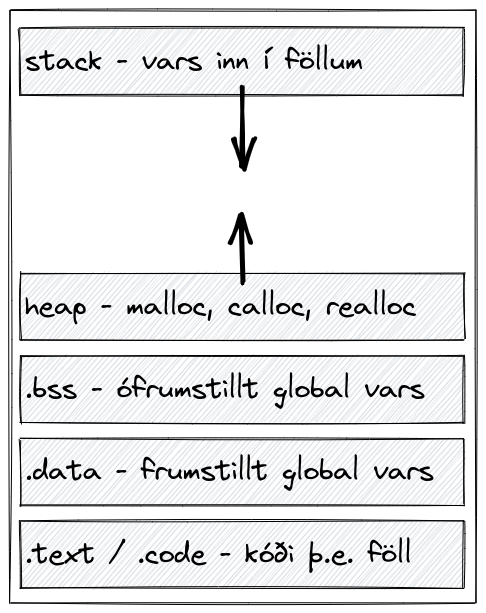
\includegraphics[scale = 0.4]{myndir/minni.excalidraw.png}

ath. global breytur sem eru skilgreindar sem 0 eða NULL eru líka í .bss
\newpage

\subsection{Sýndarminni}
\begin{itemize}
    \item sýndarvistföng: a bitar
    \item raunvistföng: b bitar
    \item síðustærð: c bæti
    \item TLB: d vítt, e sæti
    \item fjöldi mengha: f
\end{itemize}

fjöldi mengja er reiknað $\frac{e}{d} = f$

við erum með sýndarvistfang sem er 16 bitar sem skiptast í 4 mengi
þá er \textbf{VPN}$\frac{3}{4} \times 16$ bitar og \textbf{VPO} 4 bitar

\textbf{TBLT} og \textbf{TLBI} eru skipting á \textbf{VPN} og \textbf{TBLT} restin raunvistföngin eru jafn löng og \textbf{TLBT} og skipt niður í tvo hluta \textbf{PPN} og \textbf{PPO}, sem er jafn stór og \textbf{VPO}(í þessu tilfelli 4 bitar)

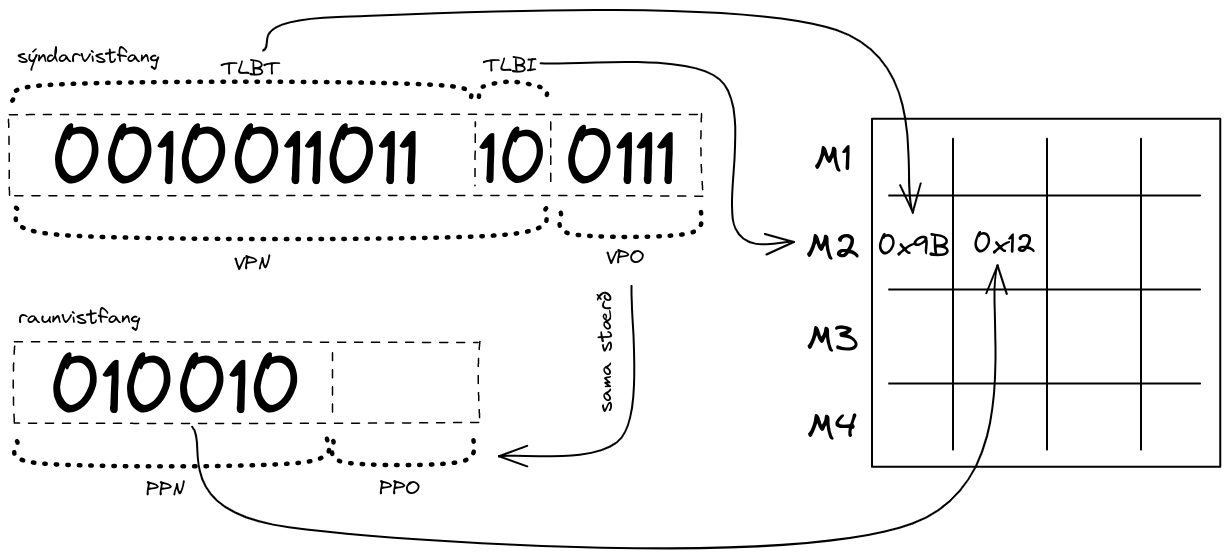
\includegraphics[scale = 0.2]{myndir/syndarminni.excalidraw.png}

annap dæmi, við erum með sýndarminni sem er 4kb að stærð, 4-vítt, E, og með 16 mengi, S, svo útfrá þessum tölum finnum við línustærð, B, með reikningnum $\frac{4096}{16 \times 4} = 64$ skiptum þessu nu upp fyrir 32-bita vistfang:

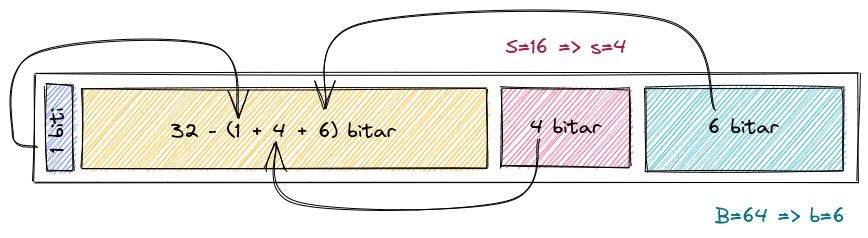
\includegraphics[scale = 0.3]{myndir/skipting.excalidraw.png}

\subsection{klukkutifsformúla}


$a + s \times r = m$
\begin{itemize}
    \item aðgangstími = a(tif)
    \item smellahlutfall = s(hlutfall)
    \item smellarefsing = r (tif)
    \item meðalaðgangstími = m (tif)
\end{itemize}

dæmi:
\begin{itemize}
    \item \text{97\%} smellahlutfall, $1 + 0.03 \times 100 = 4$
    \item \text{99\%} smellahlutfall, $1 + 0.01 \times 100 = 2$
\end{itemize}


\newpage
\section{Próf 2022 og mínar lausnir við því}
\subsection{1}
Í þessu dæmi ætlum við að nota unsigned long breytur til að tákna (allt að) 64
staka mengi (sets). Ef a er unsigned long breyta þá er stak i í menginu a ef biti i
($i = 0, \ldots 63$) er 1, annars er stak i ekki í menginu. Til dæmis væri mengið $\{0, 3\}$,
táknað með 64-bita bitastrengnum 00...01001. Athugið að bitarnir eru númeraðir frá
hægri til vinstri, svo stak 0 er í menginu, en stak 1 er ekki í menginu, stak 2 er ekki í
menginu, o.s.frv.

\subsubsection{a.}  Skrifið einnar línu fall (þ.e. bara ein \textbf{return} skipun) sem skilar sammengi
(union) tveggja slíkra mengja. Haus fallsins:
\textbf{unsigned long sammengi(unsigned long a, unsigned long b)}


\textbf{Svar}: 

\begin{lstlisting}
unsigned long sammengi(unsigned long a, unsigned long b){
    return a | b;
}
\end{lstlisting}



\subsubsection{b.}  Skrifið einnar línu fall sem skilar mengjamun (set difference) mengjanna a og b,
þ.e. öll stök sem eru í a, en ekki í b. Haus fallsins:
\textbf{unsigned long munur(unsigned long a, unsigned long b)}

\textbf{Svar}:

\begin{lstlisting}
unsigned long munur(unsigned long a, unsigned long b){
    return a & ~b;
}
\end{lstlisting}

\subsubsection{c.}  Athugið að í C er fastinn \textbf{1ul} (tölustafurinn \textbf{1} og bókstafirnir u og l) 64-bita
heiltalan 1 án formerkis. Hvaða mengi táknar segðin \textbf{($1ul << i$)}?

\textbf{Svar}:
Segðin \textbf{($1ul << i$)} táknar mengið sem inniheldur stakið i og engin önnur stök.

\subsubsection{d.}Skrifið einnar línu fall sem skilar því hvort stak i sé í menginu a. Skilagildið á
að vera 1 (\textit{satt}) ef i er í a, en 0 (\textit{ósatt}) annars. Þið megið gera ráð fyrir því að
gildið á i sé á bilinu 0 til 63. Haus fallsins:
\textbf{int stakI(unsigned long a, int i)}

\textbf{Svar}:
\begin{lstlisting}
    int stakI(unsigned long a, int i){
        return (a >> i) & 1;
    }
\end{lstlisting}

\newpage

\subsection{2}
Við höfum 10-bita fleytitölur sem fylgja IEEE staðlinum. Við vitum ekki
skiptingu þeirra í veldishluta (exp) og brothluta (frac), en það er einn formerkisbiti
fremst í þeim.

\subsubsection{a.}Hver er lágmarks bitafjöldi í brothluta fleytitölunnar til að hægt sé að tákna
töluna $3 \frac{9}{16}(=3.5625)$ nákvæmlega á þessu formi? Rökstyðjið svar ykkar með útreikningi.

\textbf{Svar}:
alright við vitum að í IEEE staðlinum erum við með fyrstu töluna sem segir til um + eða mínus næst kemur veldishlutinn og svo brothlutinn.

breytum 3.5625 í binary

\begin{align*}
    3.5625 &= 11.1001 \\
\end{align*}

setjum nú töluna í normað form ($1.f \times 2^n$) 
færum kommuna um einn stað til vinstri $1.11001 \times 2^1$ 
Veldisvísirinn er þá 1 og brothlutinn er 11001

svo Lágmarksbitafjöldi í brothlutanum er því 5 bitar


\subsubsection{b.}Hvert er bitagildið fyrir töluna $3 \frac{9}{16}(=3.5625)$ miðað við bitafjöldann fyrir brothlutann sem
þið funduð í a-lið (ef þið náðuð ekki að leysa a-liðinn megið þið gefa ykkur
raunhæft gildi bitafjöldanum fyrir brothlutann)? Sýnið útreikning á bitagildinu.


\textbf{Svar}:

þar sem við erum að vinna með 10 bita fleytitölur og við höfum að brothlutinn er 5 bitar
þá er veldishlutinn 4 bitar og formerkisbitinn er 1 biti

\begin{enumerate}
    \item Reiknum bias (skekkjustuðulinn)
    \[Bias = 2^{4-1} - 1 = 7\]
    \item Geymdur veldisvísir er þá
    \[GeymtE = E + Bias = 1 + 7 = 8\]
    8 í tvíundarkerfi er 1000
    \item setjum saman bitana:
    \begin{itemize}
        \item Formeki: 0 (jákvæð tala)
        \item Veldishlutinn: 1000
        \item Brothlutinn: 11001
    \end{itemize}

    \textbf{heildarbitaröðin og bitagildið er þá: 0 1000 11001}
\end{enumerate}



\subsubsection{c.} Segjum að í þessum 10-bita fleytitölum hefur verið ákveðið að nota einn bita
fyrir formerki, einn bita fyrir brothluta og restina af bitunum fyrir veldishlutann.
Er hægt að tákna staðlaðar tölur á þessu formi, og ef svo er, hver er þá \underline{stærsta
staðlaða talan} sem hægt er að tákna? Rökstyðjið svar ykkar.

\textbf{Svar}:
Já við getum táknað staðlaðar tölur á þessu formi 

\begin{itemize}
    \item Formerki: 1 biti
    \item Veldishlutinn: 8 bitar
    \item Brothlutinn: 1 biti
\end{itemize}


Reiknum Bias

\[2^{k-1} - 1= 2^{8-1} = 2^7 - 1 = 127\]

Hámarks veldistalan er þá $2^{8-1} - 1 = 127$

brothlutinn er 1 og við höfum gefinn 1 bita svo marktalan er 1.1 í binary sem í decimal er 1.5

stærsta staðlaða talan er því

\[1.5 \times 2^{127}\]

\subsubsection{d.} Nú hefur verið ákveðið að nota einn bita fyrir formerki, einn bita fyrir
veldishluta og restina af bitunum fyrir brothlutann. Er hægt að tákna staðlaðar
tölur á þessu formi, og ef svo er, hver er nú \underline{stærsta staðlaða talan} sem hægt er
að tákna? Rökstyðjið svar ykkar.

\textbf{Svar}:
Alright reynum þetta þá erum við með 

\begin{itemize}
    \item Formerki: 1 biti
    \item Veldishlutinn: 1 biti
    \item Brothlutinn: 8 bitar
\end{itemize}

reiknum bias

\[2^{k-1} - 1 = 2^{1-1} - 1 = 0\]

\textbf{Mögulegir veldisvísar eru þá: 0, 1}
\[E = 1 - 0 = 1\]

\textbf{Stærsta talan sem hægt er að tákna er þá:}
\[1.11111111_2 \times 2^1  = 1.(2^{1/2^1}+1/2^2+1/2^3+1/2^{\cdots}+2^8)=1.9960375 \times 2^1\]

\textbf{Stærsta staðlaða talan:}
\[1.9960375 \times 2^1 = 3.9921875\]

\newpage
\subsection{3}
Hér fyrir neðan er smalamálskóði fallsins fun:

\begin{verbatim}
    fun:
        movq    (%rdi), %rax
        jmp     .L2
    .L3:
        leaq    (%rax,%rax,2), %rax
        addq    %rax, %rax
        addq    $1, %rsi
    .L2:
        cmpq    %rdx, %rsi
        jl      .L3
        ret
\end{verbatim}


\subsubsection{a.} Hver er fjöldi vistfanga fallsins \textbf{fun} og hvert er tag hvers þeirra? Þið eigið að geta séð það út frá notkun gista í kóðanum hér að ofan. 
Rökstyðjið svarið með vísun í kóðann.


\textbf{Svar}:

Við höfum þrjár inntaksbreytur og eina staðværa breytu

\begin{itemize}
    \item \textbf{\%rdi} við sjáum að hér er \textbf{movq (rdi), rax} sem bendir til að þetta sé pointer á unsigned long gildi og fyrsta inntaksbreytan
    \item \textbf{\%rsi} Notað í samanburði \textbf{cmpq rdx, rsi} og síðan uppfærð með \textbf{addq \text{\$1}, rsi} þetta er önnur inntaksbreytan, líklega heiltala.
    \item \textbf{\%rdx} Notað í samanburði \textbf{cmpq rdx, rsi} þetta er þriðja inntaksbreytan og sennilega líka heiltala
    \item \textbf{\%rax} Notað til að geyma gildi sem er lesið úr mminni og síðan uppfært í lykkju.
\end{itemize}

því erum við með 4 vistföng

\begin{enumerate}
    \item \textbf{Bendir}: unsigned long * (í \text{\%rdi})
    \item \textbf{Heiltala s}: unsigned long (í \text{\%rsi})
    \item \textbf{Heiltala x}: unsigned long (í \text{\%rdx})
    \item \textbf{Staðvær heiltala rax}: unsigned long (í \text{\%rax})
\end{enumerate}


\subsubsection{b.}Skrifið jafngildan C kóða fyrir fallið \textbf{fun}. Þið megið velja breytunöfnin, eða
nefna þau eftir gistunum.

\textbf{Svar}:

\begin{lstlisting}
   unsigned long fun(unsigned long *ptr, unsigned long s, unsigned long x){
        unsigned long rax = *ptr;
        while(s < x){
            rax = 6 * rax;
            s = s + 1;
        }
        return rax;
    }
\end{lstlisting}


\subsubsection{c.} Smalamálskóðinn að ofan er úttak úr þýðandanum \textbf{gcc} með bestunarrofann
\textbf{-Og}. Ef notaður er bestunarrofinn \textbf{-O3} (sem er mesta mögulega bestun) fæst
kóðinn sem hér er fyrir neðan. Berið hann sama við fyrri kóðann og segið í
hvaða tilvikum \textbf{O3}-kóðinn gæti verið hraðvirkari.

\begin{verbatim}
    fun:
        movq    (%rdi), %rax
        cmpq    %rdx, %rsi
        jge     .L1
    .L3:
        leaq    (%rax,%rax,2), %rax
        addq    %rax, %rax
        addq    $1, %rsi
        cmpq    %rsi, %rdx
        jne     .L3
    .L1:
        ret

\end{verbatim}

\textbf{Svar}:
Byrjum á að skoða munin á milli þessara kóða :

við sjáum að í seinni kóðanum höfum við 
strax compare skipun í annari línu sem segir jge (jump greater or equal) sem þýðir að ef \textbf{rsi} er stærra eða jafnt og \textbf{rdx} þá er haldið áfram í \textbf{.L1} sem fer beint í return
þannig ef rsi er minna er rdx þá er farið í \textbf{.L3}

Næst fáum við leaq skipunina sem margfaldar rax með 3 og bætir í rax síðan er bætt rax við rax svo í raun er verið að gera
$6 \times rax$ síðan er 1 bætt við rsi og kannað hvort rsi sé orðið jafnt og rdx og ef ekki er farið aftur í \textbf{.L3} sem myndar lykkju.

ástæðan af hverju þetta er hraðvirkara er að það í seinna er færri hopp á milli. 



\newpage

\subsection{4}
Hér fyrir neðan er smalamálskóði fyrir endurkvæmt fall með hausinn:
\textbf{int rec(int n, int m)}:

\begin{verbatim}
    rec:
        cmpl    %esi, %edi  # lína 1
        jge     .L8         # lína 2
        movl    $0, %eax    # lína 3
        ret                 # lína 4
    .L8:
        subq    $8, %rsp    # lína 5
        addl    %esi, %esi  # lína 6
        subl    $2, %edi    # lína 7
        call    rec         # lína 8
        addl    $1, %eax    # lína 9
        addq    $8, %rsp    # lína 10
        ret                 # lína 11

\end{verbatim}

\subsubsection{a.} Sýnið jafngilt endurkvæmt C fall. Rökstyðjið einstakar skipanir út frá línum í
smalamálskóðanum.

\textbf{Svar}:

Byrjum á að skoða kóðann: 

\begin{itemize}
    \item lína 1 og 2: ef edi er stærra eða jafnt og esi þá er hoppað í \textbf{.L8}
    \item 3 og 4: ef edi er minna en esi þá er eax núllstillt og return skipun framkvæmd.
    \item lína 5: rsp er minnkað um 8
    \item lína 6: esi er tvöfaldast
    \item lína 7: edi er minnkað um 
    \item lína 8: kallað er á fallið rec
    \item lína 9: eax er hækkað um 1
    \item lína 10: rsp er hækkað um 8
    \item lína 11: return skipun
\end{itemize}

alright reynum að átta okkur á breytunum

\begin{itemize}
    \item something
\end{itemize}











\newpage
\section{Vika 1}
\large{\textbf{Kynning, Linux, C}}

\subsection{Heimadæmi spurningar}

\subsubsection{1 og 2}
kennslu aðferðir

\subsubsection{3}
Skoðið sýnidæmin á glæru 16 í fyrirlestri 1 (þ.e. $50000 * 50000$ fyrir int og $1e20 +
(-1e20 + 3.14)$ fyrir float).
\begin{itemize}
    \item[a]. Skrifið stutt forrit í Java sem prentar út niðurstöðuna úr þessum útreikningunum
(athugið að í Java eru kommutölufastar sjálfkrafa af taginu double. Til að fá
float-fasta þarf að setja f á eftir fastanum, t.d. 3.14f).
\item[b] . Reyndar er gildið 1e20 (þ.e. 1020) óþarflega stórt. Það eru til mun minni gildi
sem valda sömu vandræðum. Finnið lægsta gildi a á 10a sem gefur sömu
niðurstöðu og 1e20 í seinni formúlunni á glæru 16. Sýnið útprentun á því í Java
forriti.
\end{itemize}

\subsubsection{4}
Á glærum 20 og 21 í fyrirlestri 1 er sýnd minnisvilla sem getur komið upp í C forriti.
Útskýrið hvers vegna svona villa myndi ekki koma upp í sambærilegu Java forriti.
Hvaða kostir og gallar eru við það að leyfa möguleika á svona villum í C forritum?

\subsubsection{5}
Setjið upp linux



\newpage
\section{Vika 2}
\large{\textbf{C, Bendar, minni, notkun}}

\newpage
\section{Vika 3}
\large{\textbf{Upplýsingar sem bitar, heiltölur}}

\newpage
\section{Vika 4}
\large{\textbf{Bætaröð, fleytitölur}}

\newpage
\section{Vika 5}
\large{\textbf{Skipulag örgjava, smalamálsforritun}}

\newpage
\section{Vika6}
\large{\textbf{Stýriskipanir og stef í smalamáli}}

\newpage
\section{Vika 7}
\large{\textbf{Gögn og yfirflæði minnis}}

\newpage
\section{Vika 8}
\large{\textbf{Bestun smalamálskóða}}

\newpage
\section{Vika 9}
\large{\textbf{Minnisstigveldi, skyndiminni}}

\newpage
\section{Vika 10}
\large{\textbf{Tenging, keyrsluskrár, forritasöfn}}

\newpage
\section{Vika 11}
\large{\textbf{Frábrigði, ferlastýring}}

\newpage
\section{Vika 12}
\large{\textbf{Sýndarminni}}

\newpage
\section{Vika 13}
\large{\textbf{Minnisúthlutun, ruslasöfnun, minnisvillur}}

\newpage
\section{Vika 14}
\large{\textbf{Samantekt}}


\end{document}
